\documentclass[11pt]{article}

% --- packages (all standard on arXiv TeXLive / Overleaf) ---
\usepackage[utf8]{inputenc}
\usepackage[T1]{fontenc}
\usepackage{lmodern}
\usepackage[margin=1in]{geometry}
\usepackage{amsmath,amssymb}
\usepackage{graphicx}
\usepackage{booktabs}
\usepackage{xcolor}
\usepackage[hidelinks]{hyperref}

\title{\textbf{The Simulator Is the Oracle:\\
Quantifying Closed-Loop Verification in Automated Rocket Design}}

\author{Aaditya Edupuganti\\[2pt]
  \small Independent Researcher\\
  \small Bachelor's in Aerospace Engineering and Master's in Data Science, IIT Madras\\
  \small \texttt{github.com/aaditya4401-dot/launchloop}}

\date{\today}

\begin{document}
\maketitle

\begin{abstract}
Language-model agents are increasingly proposed for engineering design, but they
routinely assert that a design meets its requirements without ever verifying it
against a physical model. We study how much is gained by instead closing the
loop: letting a physics simulator verify every proposal and having the designer
correct itself under a bounded simulation budget. Our testbed is high-power
rocket design---choosing a motor, nose ballast, launch-rail angle, and parachute
to reach a target apogee under hard safety constraints (a waiver ceiling, a
static-stability band, and a minimum rail-exit velocity)---with RocketPy as a
ground-truth oracle. We evaluate on 100 seeded, randomized missions, bounding the
comparison below by a strong single-shot surrogate designer and above by
exhaustive search over the reachable design space. Using a deterministic
corrective policy, the closed loop attains the exhaustive-search feasibility
ceiling (solving every feasible mission) while using ${\sim}4.5\times$ fewer
simulations, and it never ships an invalid design; the single-shot baseline
commits to configurations that the simulator later invalidates on 69\% of
missions. We show that reporting apogee error alone is misleading---the
single-shot baseline appears \emph{more} accurate precisely because it ignores
the safety constraints---and argue that accuracy must always be paired with a
violation rate. We release the benchmark, the oracle-grounded evaluation harness,
and all baselines, and outline a competing-objective multi-agent LLM
instantiation for future evaluation.
\end{abstract}

\noindent\textit{\small Preprint draft. Results in this version use a
deterministic corrective policy; the competing-objective LLM instantiation is
described as framework and its empirical evaluation is future work
(Section~\ref{sec:framework}).}

\section{Introduction}

Automated design with large language models (LLMs) is advancing quickly, and a
recurring failure mode is \emph{unearned confidence}: an agent proposes a design
and declares it satisfactory without any ground-truth check. In safety-relevant
engineering---where a configuration either respects a hard constraint or does
not---this is not a stylistic flaw but a correctness one. A natural remedy is to
close the loop: verify each proposal with a trusted model of the world (a
simulator) and let the designer correct itself, iterating under a bounded budget.

This paper asks a deliberately narrow, measurable question: \textbf{how much does
closing that loop actually buy you, relative to principled baselines?} We are not
interested in demonstrating that a system ``works'' on a cherry-picked example.
We want a controlled measurement, against a lower bound (what a strong one-shot
proposal achieves) and an upper bound (what exhaustive search achieves), on a
suite of randomized problems.

Our testbed is high-power rocket flight design. Given a mission---a target
apogee, a hard waiver ceiling, a static-stability band, a minimum rail-exit
velocity, and the day's wind---a designer must choose a motor from a fixed menu,
a nose-ballast mass, a launch-rail inclination, and a main-parachute size. We use
RocketPy~\cite{rocketpy}, a validated 6-DOF trajectory simulator, as a
\textbf{ground-truth oracle}: no metric is ever accepted unless the simulator
produced it.

We make three contributions:
\begin{enumerate}
  \item A \textbf{reproducible, oracle-grounded benchmark} for closed-loop
  engineering-design methods: randomized missions, a physics oracle, and
  principled floor (single-shot) and ceiling (exhaustive-search) baselines, with
  paired statistics.
  \item A \textbf{controlled ablation} of closed-loop verification against those
  bounds, using a deterministic corrective policy so the measured effect is
  attributable to loop structure rather than to a particular reasoning engine.
  \item \textbf{Honest findings}, including a documented null result and a
  cautionary analysis of a misleading metric, plus released code.
\end{enumerate}

Our headline results, at $N = 100$ missions: the closed loop matches the
exhaustive-search feasibility ceiling at roughly a fifth of the simulation cost,
and never ships an invalid design, whereas a strong single-shot designer ships
invalid designs on 69\% of missions.

\section{Related work}

Our design sits within a 2025--2026 line of work on \emph{verifier-in-the-loop
agents}, in which a generator proposes candidates and a non-LLM evaluator scores
them inside the decision loop. \emph{Physics-in-the-Loop}~\cite{pil} embeds
validated engineering tools directly in an agent's plan--generate--evaluate--revise
cycle for CAD; \emph{Frontier-Eng}~\cite{frontiereng} formalizes a
propose--execute--evaluate loop with executable verifier feedback under a fixed
interaction budget; and the FunSearch/AlphaEvolve pattern discussed
in~\cite{feedback} pairs an LLM generator with a \emph{deterministic} evaluator
whose fitness function does not invoke another LLM. Our design shares this
structure---RocketPy is the deterministic evaluator, and we impose a hard
simulation budget---but contributes a controlled measurement of the loop's value
against explicit floor and ceiling baselines, rather than a capability
demonstration.

For multi-agent engineering design, \emph{TurboAgent}~\cite{turboagent} uses a
LangGraph supervisor with specialist agents and a physical-validation stage for
turbomachinery. Our framework (Section~\ref{sec:framework}) similarly uses
specialist agents, but with \emph{competing} objectives and an arbitrating
orchestrator; we note that the empirical results here use a deterministic policy
and defer the multi-agent evaluation to future work.

\section{Problem setup}

A \textbf{mission} specifies: a target apogee $A^\star$ and a tolerance $\tau$
(reaching within $\tau$ of $A^\star$ counts as on-target); a hard waiver
\textbf{ceiling} $C$ (apogee must not exceed it); a hard \textbf{stability band}
$[s_{\text{lo}}, s_{\text{hi}}]$ in calibers of static margin; a hard minimum
\textbf{rail-exit velocity} $v_{\min}$; and the day's \textbf{wind}.

A \textbf{configuration} is the designer's decision vector: total motor impulse
(from a fixed menu), nose-ballast mass, launch-rail inclination, and
main-parachute drag area ($c_d S$). The \textbf{oracle} flies a configuration in
RocketPy and returns apogee, static-stability margin, rail-exit velocity, and
(optionally) a landing-dispersion estimate from a small perturbed-flight
ensemble.

A configuration is a \textbf{success} iff the oracle confirms all hard
constraints (ceiling, stability band, rail-exit) \emph{and} the apogee is
on-target. Success is therefore always simulator-defined, identically for every
method compared.

\paragraph{Instantiation.} Default mission: $A^\star = 3000$~m, $\tau = 150$~m,
stability band $[1.5, 2.5]$~cal, $v_{\min} = 20$~m/s. Motor menu (total impulse,
N$\cdot$s): L900 (3500), M1540 (6000), M1920 (7500), M2310 (9000). The starting
configuration uses the largest motor, which deliberately overshoots the ceiling,
so a designer must act to succeed. Airframe geometry is fixed; the design levers
are motor, ballast, rail angle, and parachute.

\section{Method: the closed-loop designer}

The designer runs a \textbf{propose $\rightarrow$ verify $\rightarrow$ correct}
loop:
\begin{enumerate}
  \item \textbf{Verify.} The oracle evaluates the current configuration; a
  deterministic constraint check turns the metrics into a pass/fail report and an
  apogee gap.
  \item \textbf{Correct.} A policy proposes exactly one corrective change (swap
  motor, add or remove ballast, adjust rail angle, resize parachute),
  prioritizing hard-constraint repair, then closing the apogee gap.
  \item \textbf{Loop or stop.} The new configuration is re-verified. The loop
  terminates with \emph{go} when a configuration succeeds, or \emph{no-go} when
  the policy exhausts a hard budget of $B = 8$ simulations without success.
\end{enumerate}

Because every accepted design is one the oracle confirmed, the loop
\textbf{cannot ship an invalid design}: a \emph{go} is always simulator-verified,
and when no satisfying configuration is found it correctly returns \emph{no-go}.

\paragraph{Policy used in this paper.} To attribute the measured effect to loop
structure rather than to a particular reasoning engine, the results here use a
\emph{deterministic} corrective policy (repair the violated hard constraint;
otherwise step toward the target). Section~\ref{sec:framework} describes an LLM
instantiation.

\section{Baselines}

We bound the loop from both sides.

\paragraph{Single-shot (floor).} The designer receives one oracle evaluation of
the starting configuration, then commits to a single best proposal with no
further verification. To avoid a strawman, this proposal is \emph{compound and
informed}: from the one observed flight it extrapolates the impulse needed to hit
target (apogee is roughly linear in impulse) and picks the nearest menu motor.
The committed design is then audited by the oracle---the audit is a measurement,
not part of the method's budget (the designer consumed one oracle look before
committing). This isolates the value of \emph{iterating with verification} versus
making a single informed guess.

\paragraph{Exhaustive search (ceiling).} We grid-search the reachable
motor $\times$ ballast space with the oracle and keep the configuration that
satisfies the constraints and lands closest to target. This is the best result
achievable in that design space and defines \textbf{feasibility}: a mission is
feasible iff exhaustive search solves it. We report the loop-vs-single-shot
comparison both overall and on the feasible subset, so it is not diluted by
missions no method in this space could solve. (Hard constraints and on-target
depend only on the single deterministic flight, so the search runs without the
dispersion ensemble and is cheaper per mission than the loop.)

\section{Experimental setup}

\paragraph{Missions.} 100 missions from a fixed seed, each drawn as: target
apogee ${\sim}\,U[2500, 3500]$~m; ceiling $= \text{target} + U[100, 600]$~m; wind
${\sim}\,U[0, 12]$~m/s. Every method sees the same missions (a paired design).

\paragraph{Metrics.} Per mission and method: \textbf{success} (oracle-defined,
above); \textbf{hidden violation} (the method declared \emph{go} but the oracle
rejects the committed design); \textbf{oracle simulations} used to decide; and
\textbf{apogee error} $|\text{apogee} - \text{target}|$.

\paragraph{Statistics.} Because arms are paired on missions, we use McNemar's
exact test for the binary success outcome and the Wilcoxon signed-rank test for
paired apogee error, and report Wilson 95\% confidence intervals for rates. At
$N = 100$ these are still modest samples; we report them as evidence, not proof,
and flag non-significant differences explicitly.

\paragraph{Reproduce.} \texttt{make study N=100} (add \texttt{-{}-dispersion-sims 0}
for speed; the deterministic policy's decisions do not depend on dispersion) then
\texttt{python -m src.experiments.analyze}. Seed~0.

\section{A competing-objective multi-agent instantiation (framework)}
\label{sec:framework}

The corrective policy above is one instantiation of a swappable ``brain.'' The
framework also defines an LLM instantiation intended to make the objective
\emph{tension} explicit: three specialist agents, each advocating a single
objective---\textbf{performance} (hit the target apogee), \textbf{safety}
(respect the ceiling, stability band, and rail-exit floor), and
\textbf{recovery} (contain landing dispersion)---and an \textbf{orchestrator}
that reads their opinions plus the oracle-verified metrics and arbitrates the
tradeoff into the next single corrective change or a go/no-go call. A cheap ML
surrogate (an apogee predictor trained on prior flights) can pre-screen candidate
motors to rank them before a full oracle simulation, never as an accepted metric.

We stress that \textbf{the empirical results in this paper do not exercise this
instantiation}: the deterministic policy ignores specialist opinions and the
surrogate, so no claim about competing-objective arbitration or pre-screening can
be drawn from our data. Evaluating whether the multi-agent structure expands the
feasible set (e.g., by exploiting the rail-angle and parachute levers the
deterministic policy leaves fixed) and whether the surrogate reduces
simulations-to-convergence is the primary future work (Section~\ref{sec:disc}).

\section{Results}

All results: deterministic policy, $N = 100$, seed~0.

\begin{table}[h]
\centering
\small
\begin{tabular}{lccccc}
\toprule
Method & Success (95\% CI) & Feasible-subset & Hidden viol. & Mean sims & Mean apogee err \\
\midrule
Single-shot (floor)   & 31\% [23--41\%] & 89\%  & \textbf{69\%} & 1.0  & 385~m \\
\textbf{Closed loop}  & 35\% [26--45\%] & \textbf{100\%} & \textbf{0\%}  & 6.3  & 464~m \\
Exhaustive (ceiling)  & 35\% [26--45\%] & 100\% & 0\%  & 28.0 & 80~m  \\
\bottomrule
\end{tabular}
\caption{Deterministic policy over 100 randomized missions (seed 0). Of the 100
missions, 35 are feasible (solvable by exhaustive search in the
motor$\times$ballast space).}
\label{tab:results}
\end{table}

\paragraph{Finding 1---the loop matches the ceiling at a fifth of the cost.} The
closed loop solves every feasible mission (35/35), exactly matching exhaustive
search, using a mean of \textbf{6.3 simulations versus 28} (${\sim}4.5\times$
fewer). Same optimal outcome in the reachable space, far cheaper. This is our
strongest, fully empirical result.

\paragraph{Finding 2---the loop never ships an invalid design; the single-shot
ships invalid designs 69\% of the time.} The single-shot designer commits on
every mission and is wrong---the committed configuration violates a hard
constraint or misses target---on \textbf{69\%} of them, because it cannot detect
this without simulating. The loop's 0\% rate is partly by construction (it
accepts only oracle-verified designs); the empirical content is the
\emph{measured} 69\% failure rate of a strong one-shot design strategy, which
quantifies the reliability the loop provides.

\paragraph{Finding 3 (null)---the loop does not solve meaningfully more missions
than a strong single-shot.} On the feasible subset the loop solves 100\% versus
the single-shot's 89\%; it solved 4 feasible missions the single-shot missed and
none the other way. But with only 4 discordant pairs, McNemar's test gives
$p = 0.125$---not significant. We therefore do \textbf{not} claim the loop solves
more; its advantages are efficiency (Finding 1) and reliability (Finding 2).

\paragraph{A misleading metric.} Overall, the single-shot has \emph{lower} mean
apogee error (385 vs 464~m; Wilcoxon $p = 0.002$). Taken alone this suggests the
single-shot is more accurate. It is not: the single-shot aims directly at target
apogee while \emph{ignoring the hard safety constraints}---the very behavior that
produces its 69\% invalid rate---so it lands closer to target on missions where
the loop correctly refuses an unsafe design. On the feasible subset, where both
methods must also satisfy the constraints, the direction reverses (Wilcoxon
$p = 0.068$). We therefore report apogee error only alongside the violation rate,
and caution that accuracy metrics for constrained design are misleading in
isolation.

\begin{figure}[h]
\centering
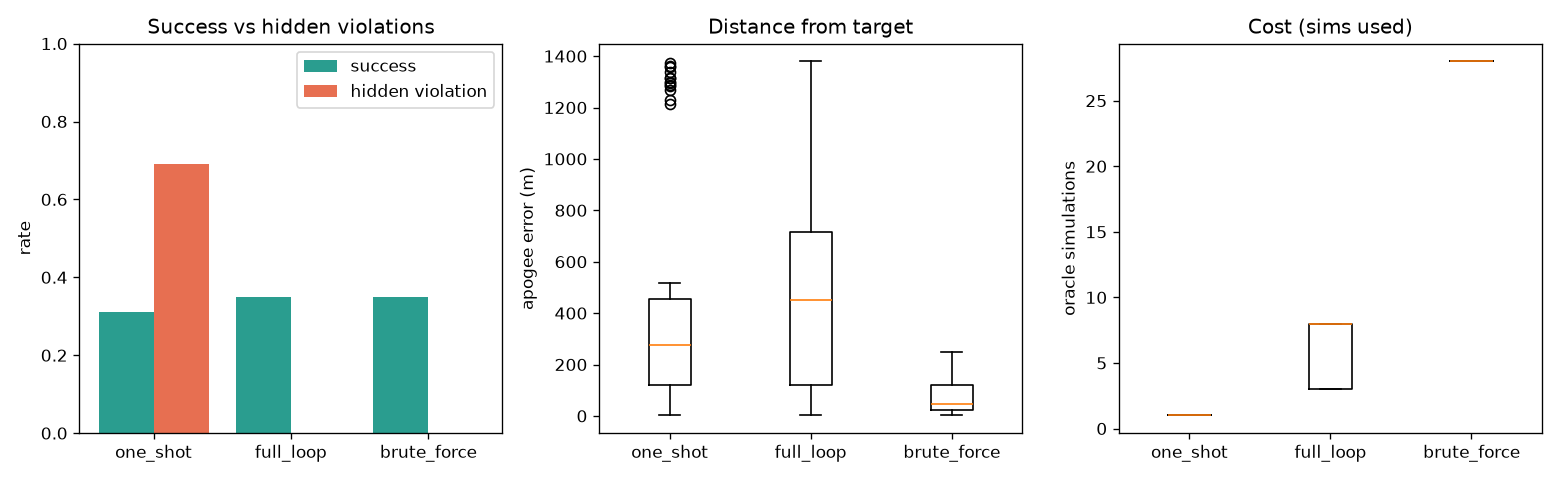
\includegraphics[width=\linewidth]{study_summary.png}
\caption{Per-arm success and hidden-violation rates (left), apogee-error
distribution (center), and simulation cost (right) over the 100 missions.}
\label{fig:summary}
\end{figure}

\section{Discussion}
\label{sec:disc}

The results draw a clean line between two kinds of value a verification loop can
provide. It did \emph{not}, with this deterministic policy, expand \emph{what}
could be solved (Finding 3): a strong single-shot already finds most feasible
designs. Its value is instead \textbf{efficiency}---reaching the exhaustive-search
optimum without exhaustive cost (Finding 1)---and \textbf{reliability}---never
committing to a design the simulator would reject (Finding 2). In a setting where
a hard-constraint violation is a safety failure, reliability is the point: the
single-shot's lower apogee error is worthless if two-thirds of its designs are
invalid.

This also suggests where an LLM instantiation could add value that the
deterministic policy cannot: by exploiting design levers the policy leaves fixed
(rail angle, parachute) and by arbitrating competing objectives, an agent might
\emph{expand the feasible set} itself---turning some of the 65 infeasible
missions feasible---which is a different and stronger claim than efficiency or
reliability. That is a direct, testable hypothesis for future work.

\section{Limitations}

\begin{itemize}
  \item \textbf{Deterministic policy, not agents.} Our empirical results use a
  fixed corrective policy; no claim about multi-agent arbitration or ML
  pre-screening is supported by this data (Section~\ref{sec:framework}).
  \item \textbf{Feasibility scope.} Feasibility is defined over
  motor$\times$ballast, the policy's reachable space; a designer that also moves
  rail angle and parachute could solve more, so our ceiling is a lower bound on
  the true one.
  \item \textbf{Oracle = evaluator.} RocketPy is both the in-loop oracle and the
  metric of success; ``success'' is simulator-relative, not flight-tested.
  \item \textbf{Narrow design space.} A synthetic four-motor menu and a single
  airframe; results may not transfer to a broader catalog.
  \item \textbf{Sample size and wind model.} $N = 100$ with a single wind model;
  differences we call non-significant may reach significance at larger $N$.
\end{itemize}

\section{Conclusion}

On a reproducible, oracle-grounded rocket-design benchmark, closing the loop with
a physics simulator lets a simple deterministic designer reach the
exhaustive-search optimum at ${\sim}4.5\times$ lower simulation cost while never
shipping an invalid design---whereas a strong single-shot designer, unable to
check itself, ships invalid designs on 69\% of missions. The loop's value here is
efficiency and reliability rather than a higher solve rate, and accuracy metrics
are misleading unless paired with a violation rate. We release the benchmark and
baselines, and identify evaluating a competing-objective multi-agent LLM
instantiation---and whether it expands the feasible set---as the primary next
step.

\paragraph{Reproducibility.} Code, benchmark, and baselines:
\url{https://github.com/aaditya4401-dot/launchloop}. All results are from
\texttt{make study N=100} (seed 0) and \texttt{python -m src.experiments.analyze}.

\begin{thebibliography}{9}

\bibitem{pil}
E.~Berger, M.~Usama, J.~Mehlst\"aubl, B.~Saske, and K.~Paetzold-Byhain.
\newblock Physics-in-the-Loop: A Hybrid Agentic Architecture for Validated CAD
Engineering Design.
\newblock arXiv:2605.19717, 2026. Accepted, IJCAI-ECAI 2026 (AI4Tech track).

\bibitem{frontiereng}
Y.~Chi, D.~Hong, D.~Jiang, et~al.
\newblock Frontier-Eng: Benchmarking Self-Evolving Agents on Real-World
Engineering Tasks with Generative Optimization.
\newblock arXiv:2604.12290, 2026.

\bibitem{feedback}
S.~Chakraborty, M.~Pourreza, R.~Sun, et~al.
\newblock On the Role of Feedback in Test-Time Scaling of Agentic AI Workflows.
\newblock arXiv:2504.01931, 2025.

\bibitem{turboagent}
J.~Du, Y.~Wu, P.~Zhao, Y.~Liu, M.~Zhang, X.~Xu, and X.~Zhang.
\newblock TurboAgent: An LLM-Driven Autonomous Multi-Agent Framework for
Turbomachinery Aerodynamic Design.
\newblock arXiv:2604.06747, 2026.

\bibitem{rocketpy}
RocketPy Team.
\newblock RocketPy: Six Degree-of-Freedom Rocket Trajectory Simulator.
\newblock \url{https://github.com/RocketPy-Team/RocketPy}.

\end{thebibliography}

\end{document}
